\documentclass[11pt]{article}
\usepackage[T1]{fontenc}
\usepackage[utf8]{inputenc}
\usepackage[english]{babel}
\usepackage{geometry}
\usepackage{fancyhdr}
\usepackage{lastpage}


%% Code listings formatting
\usepackage{listings}
\usepackage{xcolor}
\definecolor{codegreen}{rgb}{0,0.6,0}		%% comments
\definecolor{codegray}{rgb}{0.5,0.5,0.5}	%% line numbers
\definecolor{codeyellow}{rgb}{0.75,0.55,0.1}  %% strings
\definecolor{backcolour}{rgb}{1,1,1}		%% background
\lstloadlanguages{Python, bash}
\lstdefinestyle{Python}
{
	language=Python,
	backgroundcolor=\color{backcolour},
	commentstyle=\color{codegreen},
	keywordstyle=\color{magenta},
	numberstyle=\tiny\color{codegray},
	stringstyle=\color{codeyellow},
	basicstyle=\ttfamily\footnotesize,
	title=\lstname,
	breakatwhitespace=false,
	breaklines=true,
	captionpos=b,
	keepspaces=true,
	numbersep=5pt,
	showspaces=false,
	showstringspaces=false,
	showtabs=false,
	tabsize=2,
	numbers=left,
	rangebeginprefix=//\ begin:\ ,
	rangeendprefix=//\ end:\ ,
	includerangemarker=false,
	frame=lines,
	numberfirstline=false,
	firstnumber=auto
}


\lstdefinestyle{bash}
{
    backgroundcolor=\color{backcolour},
    basicstyle=\scriptsize\color{black}\ttfamily,
    frame=single,
    title=Terminal window
}


%% tikz diagram graphics
\usepackage{tikz}
\usetikzlibrary{shapes,arrows,calc,positioning}
\tikzstyle{decision} = [diamond, draw, fill=blue!20, 
    text width=4.5em, text badly centered, node distance=3cm, inner sep=0pt]
\tikzstyle{block} = [rectangle, draw, fill=blue!20, 
    text width=6em, text centered, rounded corners, minimum height=4em]
\tikzstyle{line} = [draw, -latex']
\tikzstyle{cloud} = [draw, ellipse,fill=red!20, node distance=3cm,
    minimum height=2em]


\author{
	Tolnai, Balázs András\\
 	\texttt{batol20@sdu.student.dk}
  	\and  
  	Goldapp, Christian Tim Michael\\
  	\texttt{chgol20@sdu.student.dk}
  	\and
  	Ma, Qianhua\\
  	\texttt{qima18@sdu.student.dk}
  	\and
  	Henriksen, Rasmus Aasø\\
  	\texttt{rhenr17@sdu.student.dk}
  	\and
  	Bach, Camilla Marie\\
  	\texttt{cabac19@sdu.student.dk}
}
\date{18. December 2020}
\title{%
  \textbf{Pneumonia Project} \\
  \vspace{10mm}
  \large DM873 - Deep Learning}

\pagestyle{fancy}
\fancyhead{}
\fancyfoot{}


\fancyhead[LH]{Coursecode: DM873}
\fancyhead[RH]{18. Dec 2020\\University of Southern Denmark}

\fancyfoot[LF]{github.com/??}
\fancyfoot[RF]{Page \thepage \hspace{1pt} of \pageref{LastPage}}


\begin{document}
	\maketitle
	\thispagestyle{empty}
	\vspace{1.8cm}
       	\begin{center}
       		
\includegraphics[width=0.5\textwidth]{SDU_BLACK_RGB}
       	\end{center}
	 	\vspace{1.8cm}
	\newpage
	\tableofcontents
	\newpage


	\section{Layers}

\textbf{The Dense Layer}
\\
The Dense layer implementation is quite simple. The layer inherits the layer class and takes as arguments units and an activation function. The unit parameter sets the amount of biases and weights created, as every unit is supposed to have one of each.  The activation function is set as relu as default, since this is a good all-round activation function and commonly used.  The activation function can be altered if needed.  \\
The biases are initialized with zeros because .... and the weights are initialized with a random normal function to ensure that the weights have different values.  The layer outputs the dotproduct of the input and the weights with the bias added. If an activation function is given as argument, then this is applied to the results before it is outputted. 
\\
\textbf{The Convolutional Layer}
\\
The convolutional layer takes as arguments filters, kernelsize, strides, padding, activation and dilationrate. The filters determines how many kernels is applied in each layer and is 32 by default. This value is important for the user to tune as a hyperparameter. The kernesize determines the size of each kernel to be run over the input and is 3 by 3 as default. The parameter strides is initialized to 1 by 1, and does the convolution operation without skipping pixels. The user can set activation function to be applied to the results after convolution and before output. The parameter padding is set to 'valid',  but the user can specify if they want another type of padding at the edges of the image.. The dilationrate is set to one to not do any dilution. 
\\
\textbf{The MaxPooling Layer}
\\

	%\newpage

	\section{Model}


\textbf{Data augmentation}
\newline

Data augmentation is important. Augmenting the data means (in our case) changing the pictures in a random way before showing it to the network. This way we can learn a lot more from the data at our disposal, as we are not training on the exact same images. (Ofcourse, more data would still be better). We used horizontal flip, and skipped on vertical, thinking that otherwise we would never get an image of a lung upside down. We also used zoom, rotation, shear and shift.

\textbf{The Net}
\newline
Our model is a generally quite simple model. It consists of convolution layers, followed by maxpooling layers. The filter sizes are exponentially increasing, so first we can detect larger features (like edges), and as the sizes of the feature maps get smaller, more filters can detect smaller, more detailed features. We use Batch normalization, to speed up the training time, and, perhaps reduce overfitting. We also utilised spatial dropout. Opposed to normal dropout, which is not very effective in convolutional nets, rather than dropping out individual elements, it drops out entire feature maps. This helps promote independence between feature maps. As usual, the net’s head is a fairly large dense layer.
\\\
\\\
\textbf{Training}
\newline
The training takes two iterations. First we trained the model on the training data, using validation. wet set the number of epochs to 1000, and an early stopping callback got created, to stop the training at the right moment, with a certain patience. After this, the program reads the number of epochs from history and retrains the model on the whole dataset, without validation, hopefully with better results.
	%\newpage

	\section{Evaluation}

\textbf{The Custom Data-Generator}
\\
A data-generator is conceptually simple. It is just a stream of input, through a filter/transformation, to a desired output.
For our generator specifically, we simply needed to have it read the matrix of values correctly.

\\
\textbf{The MaxPooling Layer}
\\

	%\newpage

	\section{Results}
For the very first tries we tried to make a large, VGG-16 like network. With 16 convolution layers, from 32 filters to 512, and two Dense layers. We managed to reach incredible validation accuracy.
\\\
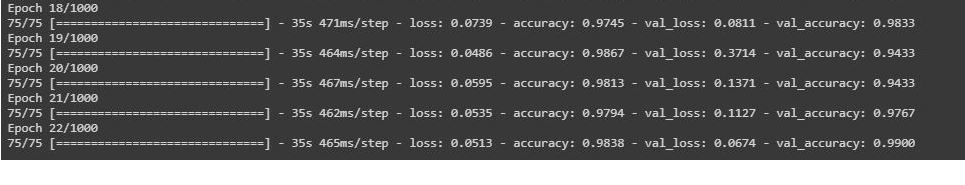
\includegraphics[scale=0.5]{over_fit_1}
\newline

\includegraphics[scale=0.5]{limitless_overfitting}
\\\
After evaluation, it turned out that it was probably just overfitting, as the model performed terrible.  It is unsure why the validation accuracy kept increasing too, perhaps the validation data was picked unluckily and was too easy to categorise compared to the training data. 
Later we tried a smaller and smaller convolutional net. We tried a net with 10 layers, double convolution layers before each pooling. This was probably still learning too quickly and start overfitting.
\\\
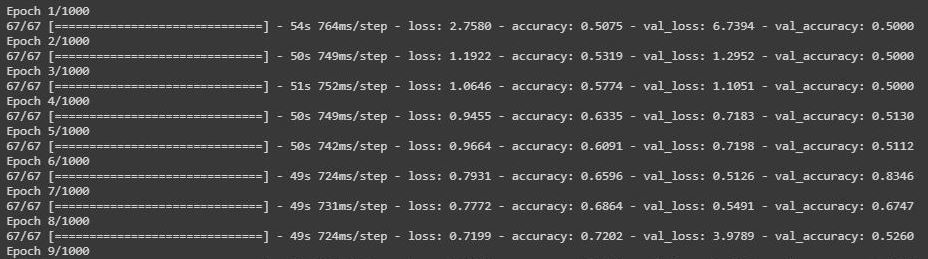
\includegraphics[scale=0.5]{double}
\\\
In the end we ended up with a simple model with single convolutional layers (filters form 64 to 1024), which performed reasonably well.
The final model's second round of training(there was no validation):
\\\
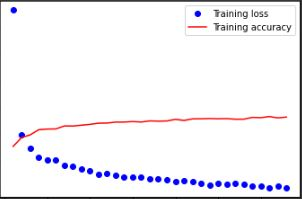
\includegraphics[scale=0.5]{long_train}
\\\
And the final evaluation:
\newline
\\\

\includegraphics[scale=0.5]{eval}

	%\newpage
	
\end{document}
